%Folgende Zeile aktivieren und als SVN property "svn:keywords" auf "Id" setzen, um SVN Versionsinformationen im Dokument zu erhalten
%\svnInfo $Id: einleitung.tex 60 2012-01-26 15:56:06Z koppor $ 

\chapter{Allgemeine Verfahren}
\label{chap:k3}
	Blablalba
	\subsection {Canny-Edge-Detektor}
		Der Canny-Edge Operator is ein von John Canny 1986 entwickelter Algorithmus zur Kantendetektion. Er liefert für ein Grauwertbild möglichst alle zusammenhängenden Kanten. Der Algorithmus gliedert sich dabei im Wesentlichen in zwei Schritte:
\begin{enumerate}
	\item Kantenhervorhebung
	\item Erzeugung von Katenzügen
\end{enumerate}

Zunächst wird das Bild mit einem zweidimensionalen Gaußkern $G$ gefaltet:
{\[\large \begin{bmatrix}
1 & 2 & 1\\ 
2 & 4 & 2 \\ 
1 & 2 & 1
\end{bmatrix}\]}
Dieser sorgt dafür, dass gröbere Störungen und Rauschen beseitigt werden.
Das gefilterte Bild wird nun auf Kanten hin untersucht. Während Flächen und Segmente in Bildern meist homogene Grauwerte besitzen, stellen Kanten große Grauwertsprünge dar. Um diese Grauwertsprünge zu detektieren, verwendet man den Sobeloperator, ein Filter, der die partiellen Ableitungen eines Pixels in $x$- und $y$-Richtung liefert. \\
Die Struktur eines 1D Sobelfilters ergibt sich dabei aus der finiten Differenz (hier: Zentraldifferenz) an der Stelle $x$:
%\begin{figure}
% 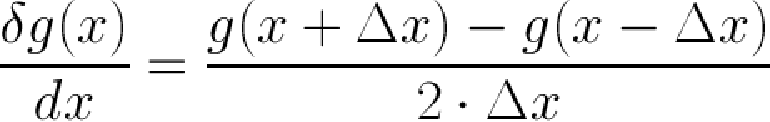
\includegraphics[width=.5\textwidth]{form1.pdf}
%\end{figure}
\begin{equation*}
\frac{\delta g(x)}{dx} = \frac{g(x + \Delta x) - g(x - \Delta x)}{2 \cdot \Delta x }
\end{equation*}
wobei $\Delta x = 1$. Damit hat der diskrete 1D Filter $S$ die Struktur
\begin{equation*}
S = \begin{bmatrix}
1 & 0 & -1
\end{bmatrix}
\end{equation*}
Erweitert auf einen zweidimensionalen Filter ergibt sich

\begin{equation*}
S(x) = \begin{bmatrix}
1 & 0 & -1\\ 
2 & 0 & -2\\ 
1 & 0 & -1
\end{bmatrix},
S(y) = \begin{bmatrix}
1 & 2 & 1\\ 
0 & 0 & 0\\ 
-1 &-2  &-1 
\end{bmatrix}
\end{equation*}

in $x$-, bzw. $y$-Richtung. \\
Die Anwendung der Filter auf das Ausgangsbild liefert die partiellen Ableitungen $G_x$ und $G_y$.
Aus diesen partiellen Ableitungen, die die Anwendung der beiden Filter liefert, lässt sich die Gradientenrichtung $d$ einer Kante berechnen:
\begin{equation*}
d(x, y) = arctan(\frac{G_y(x, y)}{G_x(x, y)})
\end{equation*}
Anschließend wird aus den partiellen Ableitungen ein Bild der absoluten Kantenstärke berechnet:
\begin{equation*}
G(x, y) = \sqrt{G_x(x, y)^2 + G_y(x, y)^2}
\end{equation*}
Im nächsten Schritt wird eine Technik names “Non-maximum suppression” angewandt, um sicherzustellen, dass Kanten nicht breiter als ein Pixel sind. Dabei werden für jedes Pixel seine 8 Nachbarn untersucht. Befindet sich in der Nachbarschaft des zu untersuchenden Pixels ein Pixel, dass einen höheren Grauwert aufweist, so wird der Grauwert des zu untersuchenden Pixels auf 0 gesetzt, es sei denn, das Pixel mit dem größeren Grauwert befindet sich entlang der Gradientenrichtung. \\ \\
Im letzten Schritt des Verfahrens werden die Pixel zu Kantenzügen zusammengefasst.
Dabei verwendet man zwei Schwellwerte $L_1 < L_2$. Zunächst wird nach einem Pixel gesucht, dessen Grauwert größer als $L_2$ ist. Dieses Pixel wird zum Startpixel des Kantenzugs erklärt. Nun wird die Kante in beiden Richtungen nach Pixel mit einem Grauwert größer $L_1$ abgesucht, welche dem Kantenzug hinzugefügt werden. Werden keine Pixel gefunden, die diese Bedingung erfüllen, bricht die Suche ab, und des wird ein neues Startpixel gesucht.Das Verfahren endet, sobald kein unmarkiertes Pixel mit einem Grauwert größer $L_2$ gefunden wird. \\ \\
Als Resultat des Verfahrens entsteht ein Bild, das eine Menge von Pixeln enthält, die idealerweise genau die Kantenpixel des Ausgangsbilds enthält.
\begin{figure}[H]
  \begin{center}
    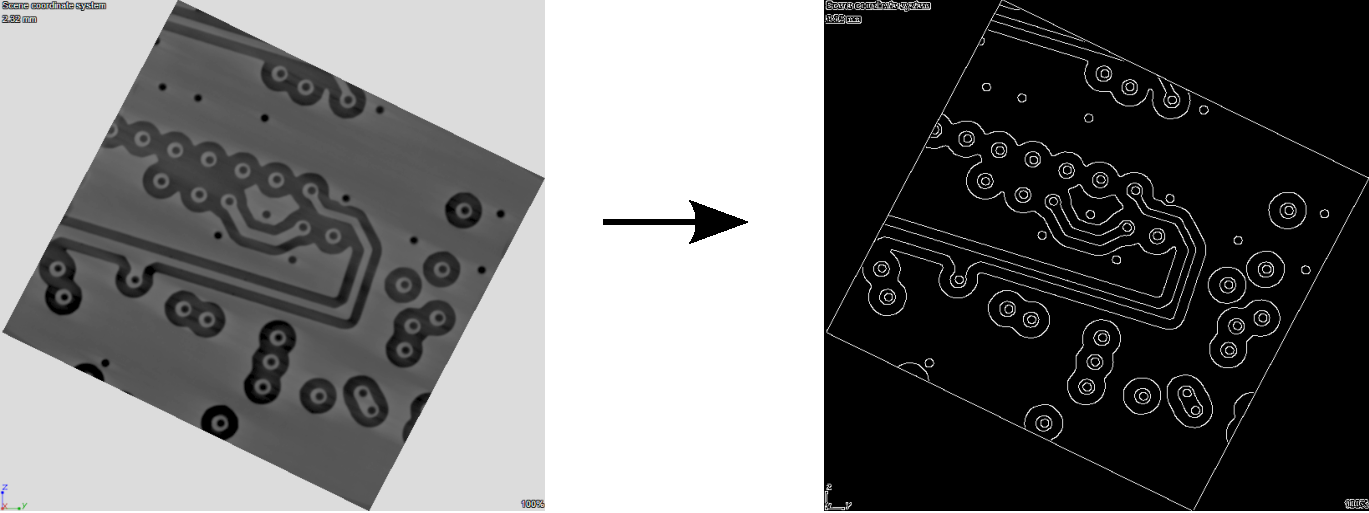
\includegraphics[width=\textwidth]{canny.pdf}
    \caption{Resultat nach der Anwendung des Canny-Edge-Detektors}
    \label{fig:dog_pyr}
  \end{center}
\end{figure}




%\vspace{-3cm}
%\vspace{2cm}



